%%%%%%%%%%%%%%%%%%%%%%%%%%%%%%%%%%%%%%%%%%%%%%%%%%%%%%%%%%%%%%%%%%%%%%%%%%%
%%%%%%%%%%%%%%%  PAGE SETUP   %%%%%%%%%%%%%%%%%%%%%%%%%%%%%%%%%%%%%%%%%%%%%
%%%%%%%%%%%%%%%%%%%%%%%%%%%%%%%%%%%%%%%%%%%%%%%%%%%%%%%%%%%%%%%%%%%%%%%%%%%
\documentclass[12pt]{article}
\usepackage{fancyhdr} %
\usepackage{setspace}
\usepackage{mathptmx}
\usepackage{graphicx}
\usepackage{amssymb}
\usepackage{epstopdf}
\usepackage{amsmath} 	
\usepackage{amssymb}
\usepackage{cite}
\usepackage{multirow}
\usepackage{wrapfig}
\usepackage{subfigure}
\usepackage{todonotes}
\usepackage{listings}
\usepackage{float}
\usepackage[nottoc,numbib]{tocbibind}
\usepackage[colorlinks=true, linkcolor=black,citecolor=black,urlcolor=blue]{hyperref}
\bibliographystyle{IEEEtran}
\DeclareGraphicsRule{.tif}{png}{.png}{`convert #1 `dirname #1`/`basename #1 .tif`.png}
\usepackage{pdfpages}
\renewcommand{\theequation}{Eq. \arabic{equation}}
\renewcommand{\abstractname}{Executive Summary}

%---------------- Letter Paper --------------------%
% be sure to change in document class too
\textwidth = 6.5 in
\textheight = 8.6 in
\oddsidemargin = 0.0 in
\evensidemargin = 0.0 in
\topmargin = 0.0 in
\headheight = 0.0 in
\headsep = 0.2in
\parskip = 0.2in
\parindent = 0.0in

%%%%%%%%%%%%%%%%%%%%%%%%%%%%%%%%%%%%%%%%%%%%%%%%%%%%%%%%%%%%%%%%%%%%%%%%%%%%
%%%%%%%%%%%%%%%  COVER PAGE   %%%%%%%%%%%%%%%%%%%%%%%%%%%%%%%%%%%%%%%%%%%%%%
%%%%%%%%%%%%%%%%%%%%%%%%%%%%%%%%%%%%%%%%%%%%%%%%%%%%%%%%%%%%%%%%%%%%%%%%%%%%
\begin{document}
\thispagestyle{empty}
\begin{center}
\vspace*{1.25in}
{\LARGE \textbf{Inline Tech Injection Pump}} %<---- Insert your project title here

{\Large Team BANTA\\ Spring 2018\\ \vspace*{0.1in}Submitted to: Dr. Yonas Niguse}

\vspace{1.0in}

% author names and CLIDS
\begin{figure}[!h]
\begin{minipage}{0.45\textwidth}
\begin{center}
Nick Beall \\
Department of Mechanical Engineering\\
University of Louisiana at Lafayette\\
Lafayette, LA 70504\\
{\tt neb2121@louisiana.edu}
\end{center}
\end{minipage}
%%
\hspace{0.08\textwidth}
\begin{minipage}{0.45\textwidth}
\begin{center}
Andrew Boudreau \\
Department of Mechanical Engineering\\
University of Louisiana at Lafayette\\
Lafayette, LA 70504\\
\tt{akb5741@louisiana.edu}
\end{center}
\end{minipage}
\end{figure}
%
\vspace{0.2in}
\begin{figure}[!h]
\begin{minipage}{0.45\textwidth}
\begin{center}
Tyler LaCombe \\
Department of Mechanical Engineering\\
University of Louisiana at Lafayette\\
Lafayette, LA 70504\\
{\tt tll6118@louisiana@edu}
\end{center}
\end{minipage}
%%
\hspace{0.08\textwidth}
\begin{minipage}{0.45\textwidth}
\begin{center}
Alex Simpson \\
Department of Mechanical Engineering\\
University of Louisiana at Lafayette\\
Lafayette, LA 70504\\
\tt{ats6547@louisiana.edu}
\end{center}
\end{minipage}
\end{figure}
%%%
\vspace{0.2in}
\begin{figure}[!h]
%\begin{minipage}{0.45\textwidth}
\begin{center}
Blake Talbot\\
Department of Mechanical Engineering\\
University of Louisiana at Lafayette\\
Lafayette, LA 70504\\
{\tt bxt8092@louisiana.edu}
\end{center}
%\end{minipage}
\end{figure}


\end{center}
%%%%%%%%%%%%%%%%%%%%%%%%%%%%%%%%%%%%%%%%%%%%%%%%%%%%%%%%%%%%%%%%%%%%%%%%%%%
%%%%%%%%%%%%%%%  SIGNATURE PAGE   %%%%%%%%%%%%%%%%%%%%%%%%%%%%%%%%%%%%%%%%%
%%%%%%%%%%%%%%%%%%%%%%%%%%%%%%%%%%%%%%%%%%%%%%%%%%%%%%%%%%%%%%%%%%%%%%%%%%%
%
\newpage
\thispagestyle{empty}

\doublespacing 
\begin{figure}[!h]
\begin{minipage}{0.45\textwidth}
\begin{flushleft}
{\bf Blake Talbot}\\
\vspace{.3in}
Signature:\hrulefill \\
\vspace{.3in}
Date: \hrulefill \\
\end{flushleft}
\end{minipage}
%%
\hspace{0.08\textwidth}
\begin{minipage}{0.45\textwidth}
\begin{flushleft}
{\bf Andrew Boudreau} \\
\vspace{.3in}
Signature:\hrulefill \\
\vspace{.3in}
Date: \hrulefill \\
\end{flushleft}
\end{minipage}
\end{figure}
%
\vspace{0.6in}
\begin{figure}[!h]
\begin{minipage}{0.45\textwidth}
\begin{flushleft}
{\bf Nick Beall} \\
\vspace{.3in}
Signature:\hrulefill \\
\vspace{.3in}
Date: \hrulefill \\
\end{flushleft}
\end{minipage}
%%
\hspace{0.08\textwidth}
\begin{minipage}{0.45\textwidth}
\begin{flushleft}
{\bf Tyler LaCombe} \\
\vspace{.3in}
Signature:\hrulefill \\
\vspace{.3in}
Date: \hrulefill \\
\end{flushleft}
\end{minipage}
\end{figure}
%%%
\vspace{0.6in}
\begin{figure}[!h]
\begin{minipage}{0.45\textwidth}
\begin{flushleft}
{\bf Alex Simpson} \\
\vspace{.3in}
Signature:\hrulefill \\
\vspace{.3in}
Date: \hrulefill \\
\end{flushleft}
\end{minipage}
\end{figure}

%%%%%%%%%%%%%%%%%%%%%%%%%%%%%%%%%%%%%%%%%%%%%%%%%%%%%%%%%%%%%%%%%%%%%%%
%%%%%%%%%%%%%%%  EXECUTIVE SUMMARY  %%%%%%%%%%%%%%%%%%%%%%%%%%%%%%%%%%%
%%%%%%%%%%%%%%%%%%%%%%%%%%%%%%%%%%%%%%%%%%%%%%%%%%%%%%%%%%%%%%%%%%%%%%%
\newpage
\thispagestyle{empty}
\begin{abstract}
\vspace{-0.2in}
\doublespacing
\hspace{0.5in}The project consisted of obtaining a solution to minimize operating cost of field equipment currently being powered by solar power units or batteries, which is costly for pipeline companies. The solution was to design a turbine that would be inserted into the pipeline and the flow of the fluid in the pipe would rotate a shaft to power a generator to charge the batteries or directly supply power to the equipment. The solution would cause a significant drop in operating cost. Different blade designs were created for the turbine to determine which would be best suited for the given specifications. CFD analysis was conducted to be able to select the most appropriate blade design. After the CFD analysis, power calculations were conducted to conclude if the design would generate enough power to charge the batteries. The results showed that the amount of power required would be 72 watts and the amount of power obtained from the design would be approximately 1,400 watts. The design provided more than enough power to charge the batteries and also would have enough power generated to power any nearby equipment. The results show that this design would be a plausible source of power for any nearby equipment along the pipeline.
\end{abstract}
%
%%%%%%%%%%%%%%%%%%%%%%%%%%%%%%%%%%%%%%%%%%%%%%%%%%%%%%%%%%%%%%%%%%%%%%%
%%%%%%%%%%%%%%%  TABLE OF CONTENTS  %%%%%%%%%%%%%%%%%%%%%%%%%%%%%%%%%%%
%%%%%%%%%%%%%%%%%%%%%%%%%%%%%%%%%%%%%%%%%%%%%%%%%%%%%%%%%%%%%%%%%%%%%%%
\newpage
\thispagestyle{empty}
\tableofcontents
%
%
%
%
%
%
%
%%%%%%%%%%%%%%%%%%%%%%%%%%%%%%%%%%%%%%%%%%%%%%%%%%%%%%%%%%%%%%%%%%%%%%%
%%%%%%%%%%%%%%%  GOALS  %%%%%%%%%%%%%%%%%%%%%%%%%%%%%%%%%%%%%%%%%%%%%%%
%%%%%%%%%%%%%%%%%%%%%%%%%%%%%%%%%%%%%%%%%%%%%%%%%%%%%%%%%%%%%%%%%%%%%%%
\newpage
% \setcounter{page}{1} % reset the page counter, so it begins with the page of the introduction section
% \section{Goals}
% \label{sec:goals}
% \vspace{-0.2in}
% \doublespacing

% \hspace{0.5 in}The project's overall goal is to conclude the feasibility of this project, along with defining the boundaries and conditions at which this concept is optimal.
% The overall success of this project includes the design, proof, and implementation of a vertical axis turbine that has the capabilities to extract power from a flowing natural gas pipeline and convert it to mechanical energy. The extracted power would be used to replace batteries currently being used to power any necessary equipment that is used in a downstream pipeline setup. As of now companies potentially spend an unnecessary amount of money replacing batteries every year. Providing a cheaper alternative to supply power to companies has potential to be both innovative and lucrative.  
%%%%%%%%%%%%%%%%%%%%%%%%%%%%%%%%%%%%%%%%%%%%%%%%%%%%%%%%%%%%%%%%%%%%%%%
%%%%%%%%%%%%%%%  INTRODUCTION/ BACKGROUND  %%%%%%%%%%%%%%%%%%%%%%%%%%%%
%%%%%%%%%%%%%%%%%%%%%%%%%%%%%%%%%%%%%%%%%%%%%%%%%%%%%%%%%%%%%%%%%%%%%%%
\setcounter{page}{1}
\vspace{-0.2in}
\section{Introduction/ Background}
\label{sec:intro}
\vspace{-0.2in}
\doublespacing

\hspace{0.5 in}The entirety of this project includes the design, proof, and implementation of a vertical axis turbine that has the capabilities to extract power from a flowing natural gas pipeline and convert it to mechanical energy. The extracted power would be used to replace batteries currently being used to power any necessary equipment that is used in a downstream pipeline system. As of now, companies potentially spend an unnecessary amount of money replacing batteries every year. Providing a cheaper alternative to supply power to companies has potential to be both innovative and lucrative.
% Prior to acquiring the project, Stonewall completed preliminary calculations. It was agreed upon that these results must be checked, and not duplicated unless absolutely necessary for the overall success of the project. Some communication was made between knowledgeable sources working in the industry to gather an accurate estimate of flow rate at the wellhead, injection pumps being used, and pressures at the location of the pump. This concept was awarded a patent prior to the acquisition of negotiations with Stonewall. A main functionality difference from existing patents in the same area of interest is the ability to be retracted after the installment of the inline turbine generator. This can be for a number of reasons including, but not limited to, maintenance of the pipeline or the turbine, and the possibility to uninstall the turbine in order to bleed pressure off from the existing pipeline.
%%%%%%%%%%%
% \hspace{0.5 in}Initially, the design was to be inserted horizontally through a 2 inch ball valve at an elbow in piping, but in the beginning of the semester, the customer changed that requirement to being inserted into a 1 inch weldolet. This was a drastic modification to the parameters due to the design orientation. 
%%%%%%%%%%%
% Due to the nature of the project, a major concern was maintaining overall efficiency of the pipeline. The conservation of energy indicates the location of the device is critical. The device must be placed near the wellhead where pressure is abundant from the natural reservoir. Normally, pressure reducers or orifices are placed in this general location because of excessive fluid pressure coming from the reservoir. The device being designed can replace the pressure reducers or orifices, and serve as a way of harnessing essentially free energy.
%%%%%%%%%%%
% \hspace{0.5 in}Preliminary research has shown that in order to maximize power generated from the fluid, multiple design parameters must be optimized. Designs favor a savonius vertical axis wind turbine (VAWT), and a spherical two and three blade model with the NACA-0012 airfoil, with flow being perpendicular to the device. While it may seem that the design concepts are being limited, the variables and parameters of each can drastically fluctuate and result in several different designs. An example of this can be seen by looking at the lone component of the blades. Parameters such as angle of attack, angle of twist, number of blades, and orientation are taken into account.
%%%%%%%%%%%%%%%%%%%%%%%%%%%%%%%%%%%%%%%%%%%%%%%%%%%%%%%%%%%%%%%%%%%%%%%
%%%%%%%%%%%%%%%  DESIRED END PRODUCT  %%%%%%%%%%%%%%%%%%%%%%%%%%%%%%%%%
%%%%%%%%%%%%%%%%%%%%%%%%%%%%%%%%%%%%%%%%%%%%%%%%%%%%%%%%%%%%%%%%%%%%%%%
%% Identify the nature and function of the end-product desired. 
\vspace{-0.2in}
\section{Desired End Product}
\label{sec:End Product}
\vspace{-0.2in}
\doublespacing

\hspace{0.5 in}Ideally, at the conclusion of the semester, a retractable turbine generator would be provided and would satisfy the design parameters and output requirements assigned by the customer. The devices blades must be able to convert the fluid's work from the flow conditions to mechanical shaft work. This shaft work will then be converted to electrical energy through the means of a generator in order to supply energy for a chemical injection pump, or any related field equipment near the insertion point. The overall goal for the product is to provide oil companies with an alternative, less expensive method to power their equipment. 
%%%%%%%%%%%%%%%%%%%%%%%%%%%%%%%%%%%%%%%%%%%%%%%%%%%%%%%%%%%%%%%%%%%%%%%
%%%%%%%%%%%%%%%  DESIRED REQUIREMENTS  %%%%%%%%%%%%%%%%%%%%%%%%%%%%%%%%
%%%%%%%%%%%%%%%%%%%%%%%%%%%%%%%%%%%%%%%%%%%%%%%%%%%%%%%%%%%%%%%%%%%%%%%
%
% List detailed design and function requirements and specifications.
%
\vspace{-0.2in}
\section{Desired Requirements}
\label{sec:Requirements}
\vspace{-0.2in}
\doublespacing

\hspace{0.5 in}Design requirements such as dimensions, desired power output, providing a seal to the surrounding environment, and being able to retract the turbine in and out of the pipeline were given both from Stonewall and Enbridge. The pipeline is specified as a 3 inch pipe with natural gas as flowing fluid that has a 1 inch weldolet as an insertion point, which is perpendicular to the flow direction. The turbine generator will rotate due to fluid flow of the natural gas in the pipeline to generate shaft work, which will then be converted to electrical power. The electrical power required to maintain operation for the chemical injection pump is around 72 Watts. During insertion, the pipeline must remain sealed to prevent any leakage of the natural gas into the environment. 
\vspace{-0.2in}
%%%%%%%%%%%%%%%%%%%%%%%%%%%%%%%%%%%%%%%%%%%%%%%%%%%%%%%%%%%%%%%%%%%%%%%
%%%%%%%%%%%%%%%  TECHNICAL APPROACH   %%%%%%%%%%%%%%%%%%%%%%%%%%%%%%%%%
%%%%%%%%%%%%%%%%%%%%%%%%%%%%%%%%%%%%%%%%%%%%%%%%%%%%%%%%%%%%%%%%%%%%%%%
%
% Describe overall approach for the problem. Discuss steps completed and the outcome, and identify those remaining.
%
\section{Technical Approach}
\label{sec:Approach}
\vspace{-0.2in}
\doublespacing

\hspace{0.5 in}The scope of work introduced in August 2017, was substantially revised in January 2018. Stonewall was approached by a potential customer who wished to change the insertion orientation of the turbine inside the pipeline. Initially, turbine blades were to be inserted horizontally into a 2 inch pipe and changed to a vertical insertion in a 3 inch pipeline through a 1 inch weldolet. This caused for a complete restart in the design process. The approach that is to be discussed covers everything completed on the new design requirements.

\hspace{0.5 in}In order to solve this problem, an overall understanding of the project was needed. Various research papers dealing with harnessing power through the means of a vertical axis turbine were read to give clarity to the basic theories and principles needed to be considered \cite{research}\cite{Fluids}. Pipeline conditions given by a contact through Stonewall can be seen in Table 1, found in the Appendix. This information was used in correlation with a multitude of fundamental equations that will be shown when discussing the process.

\hspace{0.5 in}The complexity of Inline Tech and the initial lack of knowledge regarding the CFD software caused for a more simple, steady-flow CFD analysis to be ran, rather than a complex transient analysis. This is largely in part to convolution introduced in the analysis due to moving parts. Time spent learning how to use the software, as well as check the accuracy of the results, took the majority of the semester. Normally, CFD analysis are time consuming and require a computer with plenty RAM and computing power, but Autodesk allows for student to solve the analysis on the cloud for free.

\hspace{0.5 in}Flow rate was converted from standard cubic feet per minute (SCFM) to actual cubic feet per minute (ACFM) using (\ref{eqn:SCFM}) below.
%%%%%%%%%%%%%%%%%%%%%
 \begin{equation}
{ACFM} = {SCFM}({\frac{1 atm}{P_{in}+1 atm}})(\frac{T_{act} [R]}{60^{o}F})
\label{eqn:SCFM}
\end{equation}
%%%%%%%%%%%%%%%%%%%%%
The density of the natural gas was computed using the ideal gas law, shown in \ref{eqn:rho} below. Both of these determined values, along with the temperature of the gas, were used as boundary conditions within the CFD setup.
%%%%%%%%%%%%%%%%%%%%%
\begin{equation}
\rho_{gas} = \frac{P_{in}}{R_{g}T} 
\label{eqn:rho}
\end{equation}
%%%%%%%%%%%%%%%%%%%%%
\hspace{0.5 in}Deciding the boundary conditions of the inlet and outlet was challenging to determine for the sake of accuracy. In order to account for this, two separate scenario's were analyzed for each design. The first scenario was defined by pressure and temperature boundary conditions at the inlet, and volume flow rate at the outlet. The second scenario was defined by the volume rate and temperature boundary conditions at the inlet, while pressure was applied to the outlet. Realistically, mass flow rate entering the system should be equal to the mass flow rate exiting the system, so in order to determine which scenario was most accurate, bulk results from the analysis were observed. The bulk results showed the mass flow rates entering and exiting the system were nearly identical for the first scenario, but differed for scenario two by approximately 3 to 4 $\frac{lbm}{s}$. This was due to the outlet only being defined by a pressure, and not direction of flow. This allowed for a swirling effect to occur at the outlet, and thus mass re-entering into the system, causing a mass imbalance. 

\hspace{0.5 in}Prior to actually running the analysis, the mesh was the defined, and program features allowed for mesh adaption to be implemented during the solving process. This would allow for the program to adapt the mesh in critical areas based off of an internal algorithm, and thus increasing the accuracy of the analysis. The mesh size is imperative to the results of the analysis. Large mesh size causes for shorter solving times, but the trade off is skewed results. Oppositely, a smaller mesh size implements very accurate results, but the trade off is the amount of time taken to solve the analysis. Because of Autodesk's cloud solving capabilities, it allowed for the mesh size to be relatively small, and still solve the analysis in a reasonable amount of time. The mesh for the fluid volume and the blades can be seen in Figure \ref{VFM} and \ref{Fig:BM}.\\

%%%%%%%%%%%%%%%%%%%%%
% \vspace{25pt}

\begin{figure}[ht]
\begin{minipage}{0.5\textwidth}
\begin{center}
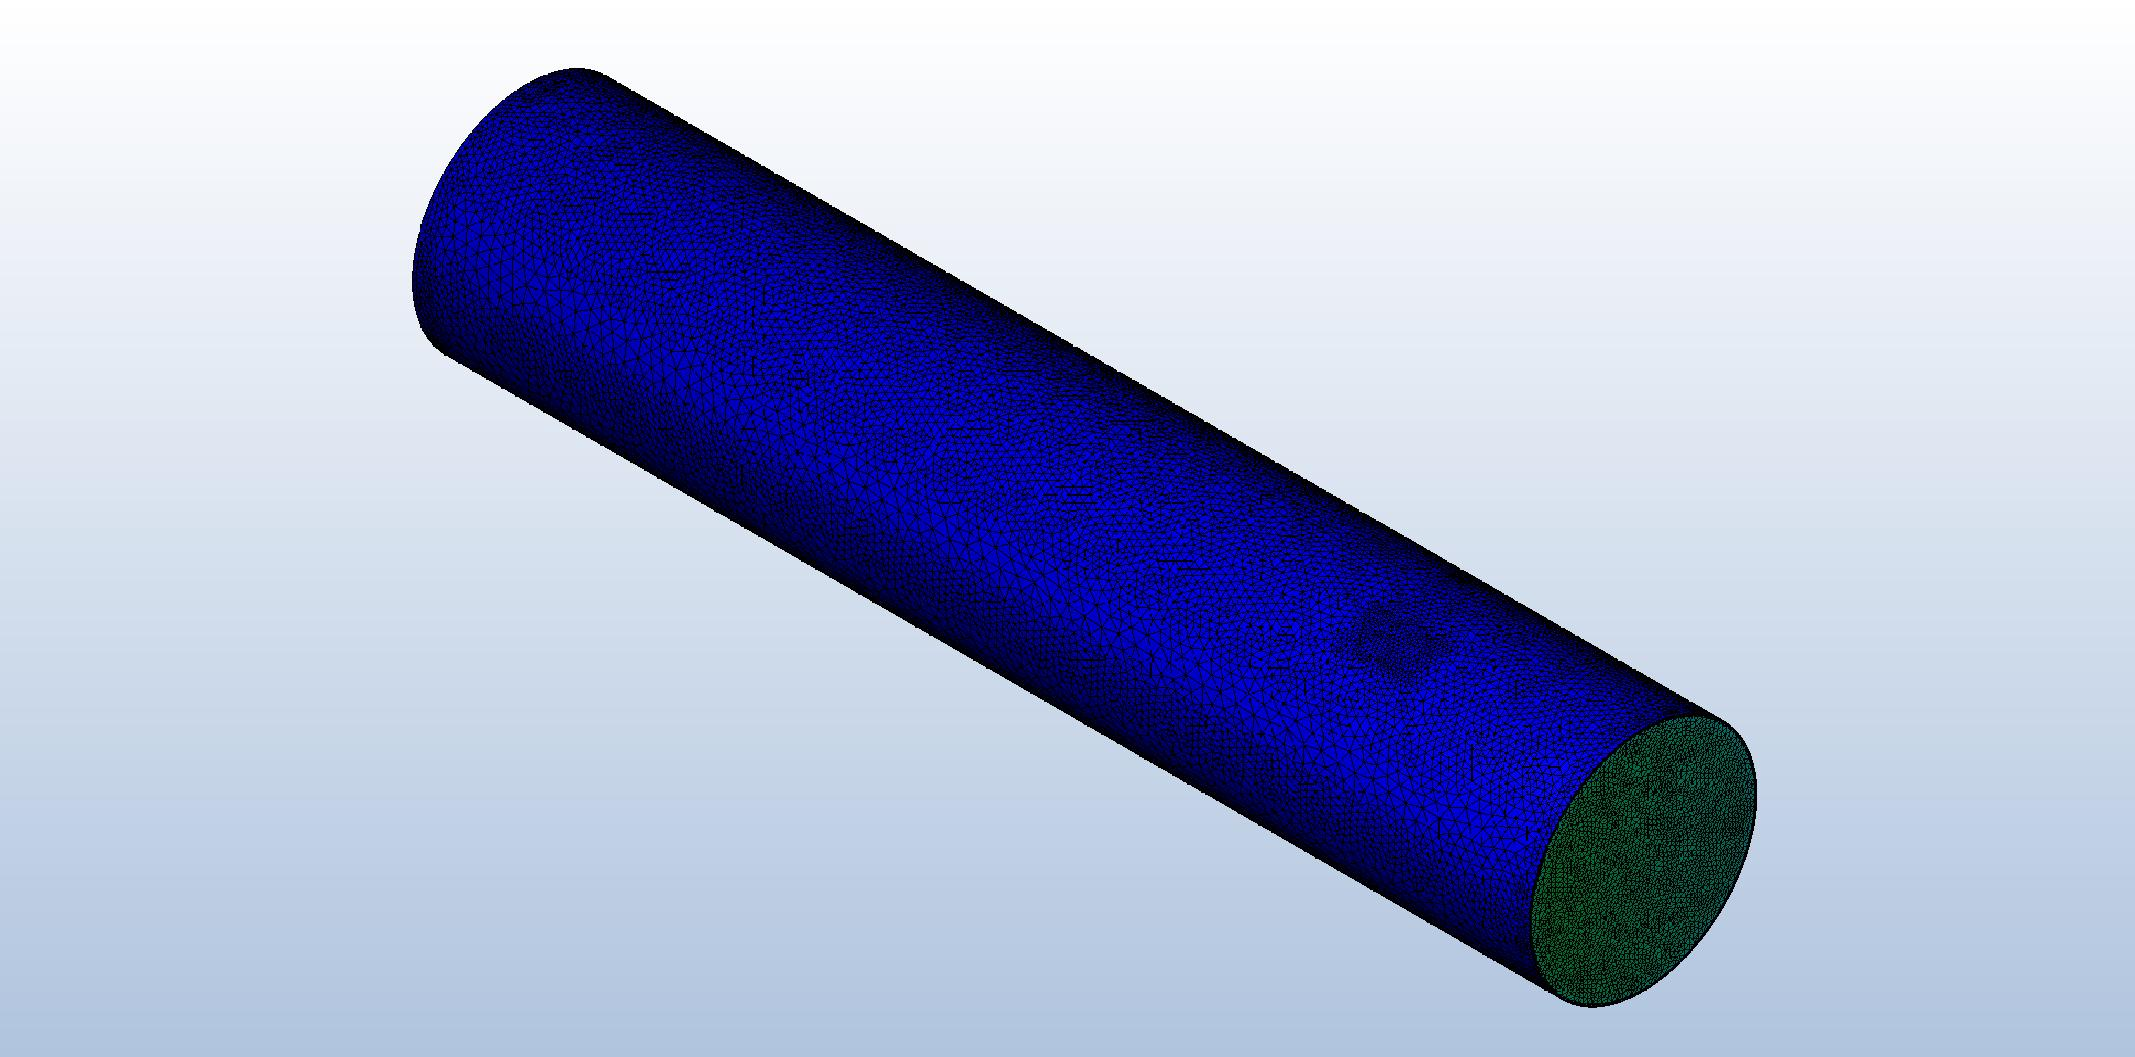
\includegraphics[width=0.75\textwidth]{Fluid_Volume_Mesh}
\caption[p1] {Mesh generated for the fluid volume}
\label{VFM}
%\vspace{-0.4in}
\end{center}
\end{minipage}
\begin{minipage}{0.5\textwidth}
\begin{center}
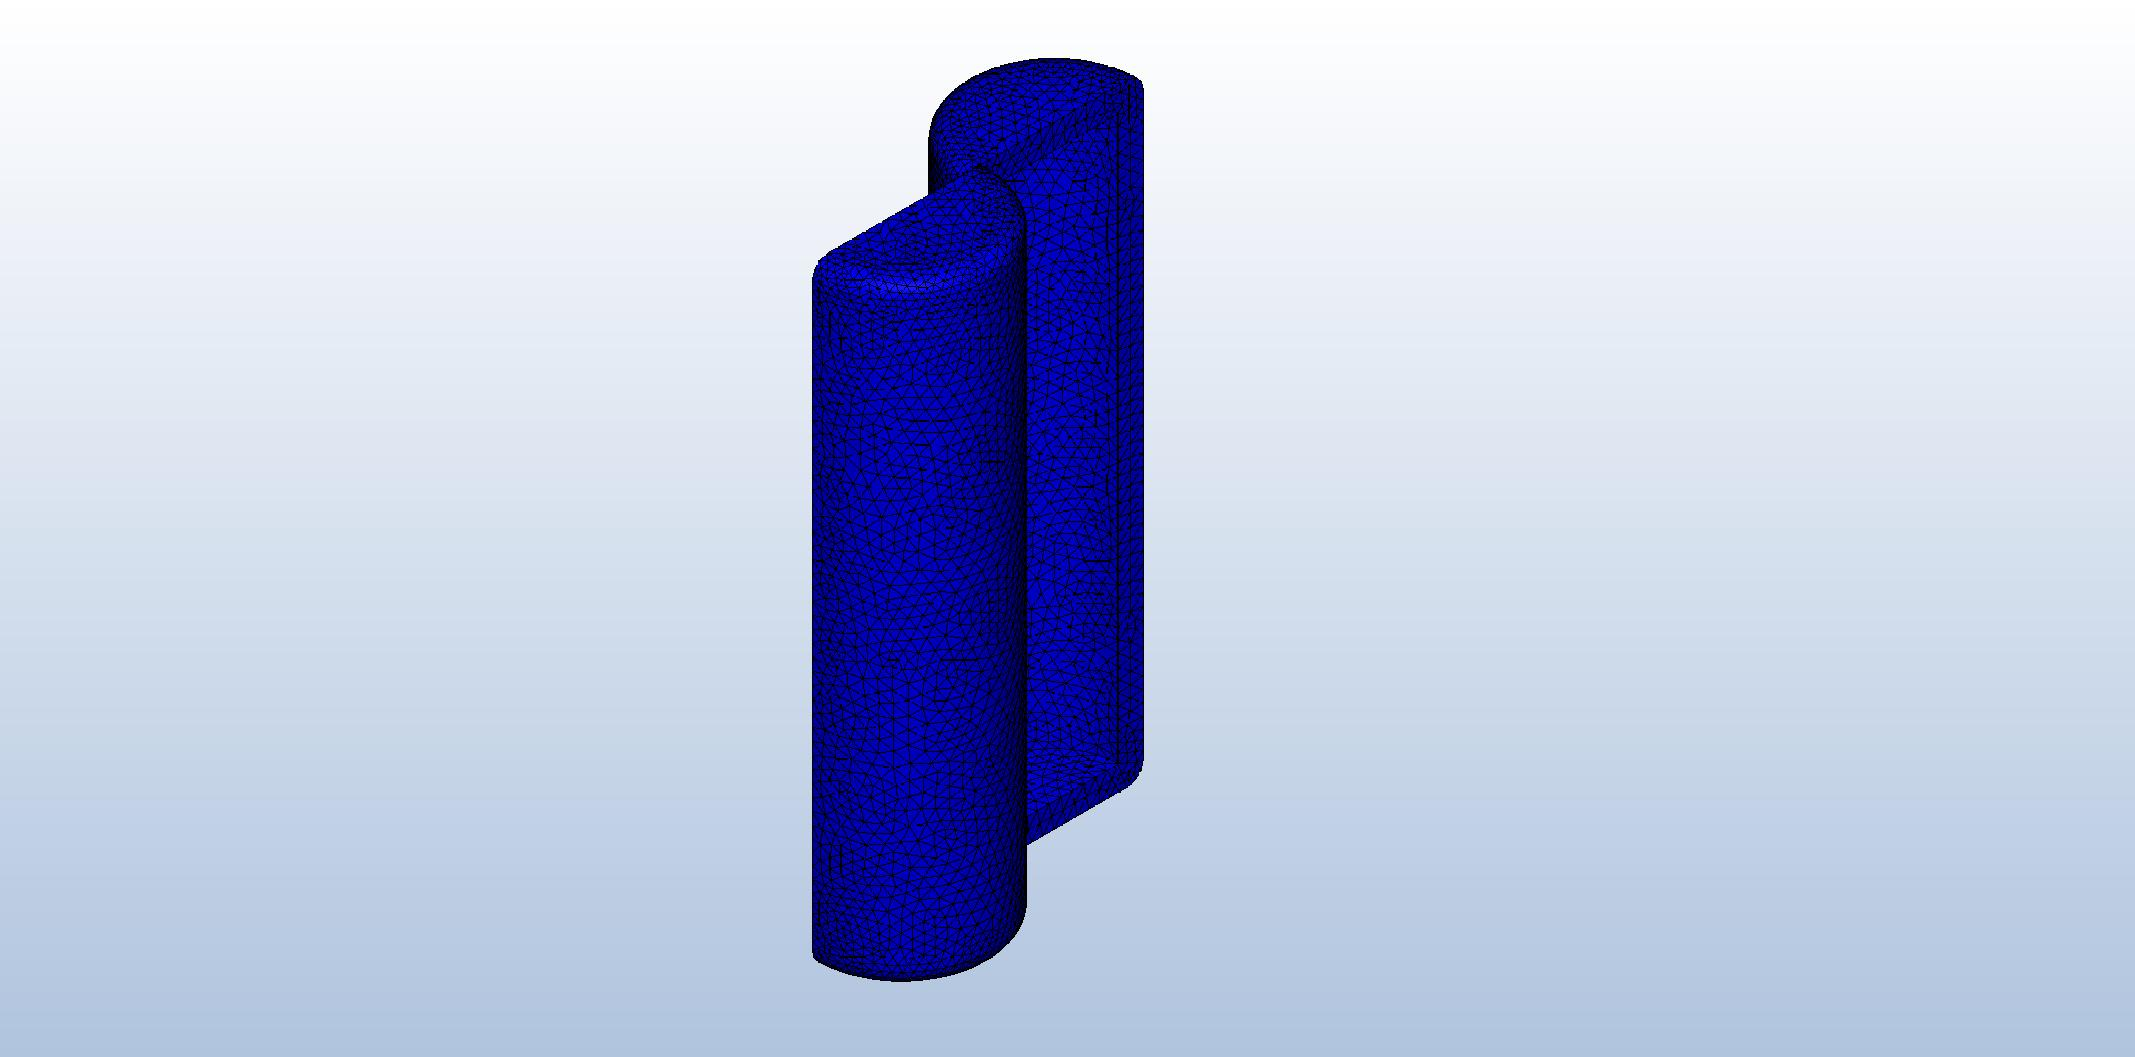
\includegraphics[width=0.75\textwidth]{Blade_Mesh}
\caption[p1] {Mesh generated for the blades}
\label{Fig:BM}
\end{center}
\end{minipage}
\end{figure}
%%%%%%%%%%%%%%%%%%%%%%%%%%%%%%%%%%%%%%%%%%%%%%%%%%%%%%%%%%%%%%%
%%%%%%%%%%%%%%%%%%%%%%%%%%%%%%%%%%%%%%%%%%%%%%%%%%%%%%%%%%%%%%%
%%%%%%%%%%%%%%%%%%%%%%%%%%%%%%%%%%%%%%%%%%%%%%%%%%%%%%%%%%%%%%%
\hspace{0.5 in}Once the analysis was solved, results could be observed and extracted through a combination of plane results and bulk results. Plane results for the velocity magnitudes across the length of the pipe, normal to the z-axis, for the Simple Savonius design are shown in Figures \ref{ssv} and \ref{ssp} and for the Crescent Savonius design in Figures \ref{cvm} and \ref{cp}.
\\
%%%%%%%%%%%%%%%%%%%%%%%%%%%%%%%%%%%%%%%%%%%%%%%%%%%%%%%%%%%%%%%
%%%%%%%%%%%%%%%%%%%%%%%%%%%%%%%%%%%%%%%%%%%%%%%%%%%%%%%%%%%%%%%
%%%%%%%%%%%%%%%%%%%%%%%%%%%%%%%%%%%%%%%%%%%%%%%%%%%%%%%%%%%%%%%
% % \vspace{25pt}
\begin{figure}[H]
\begin{center}
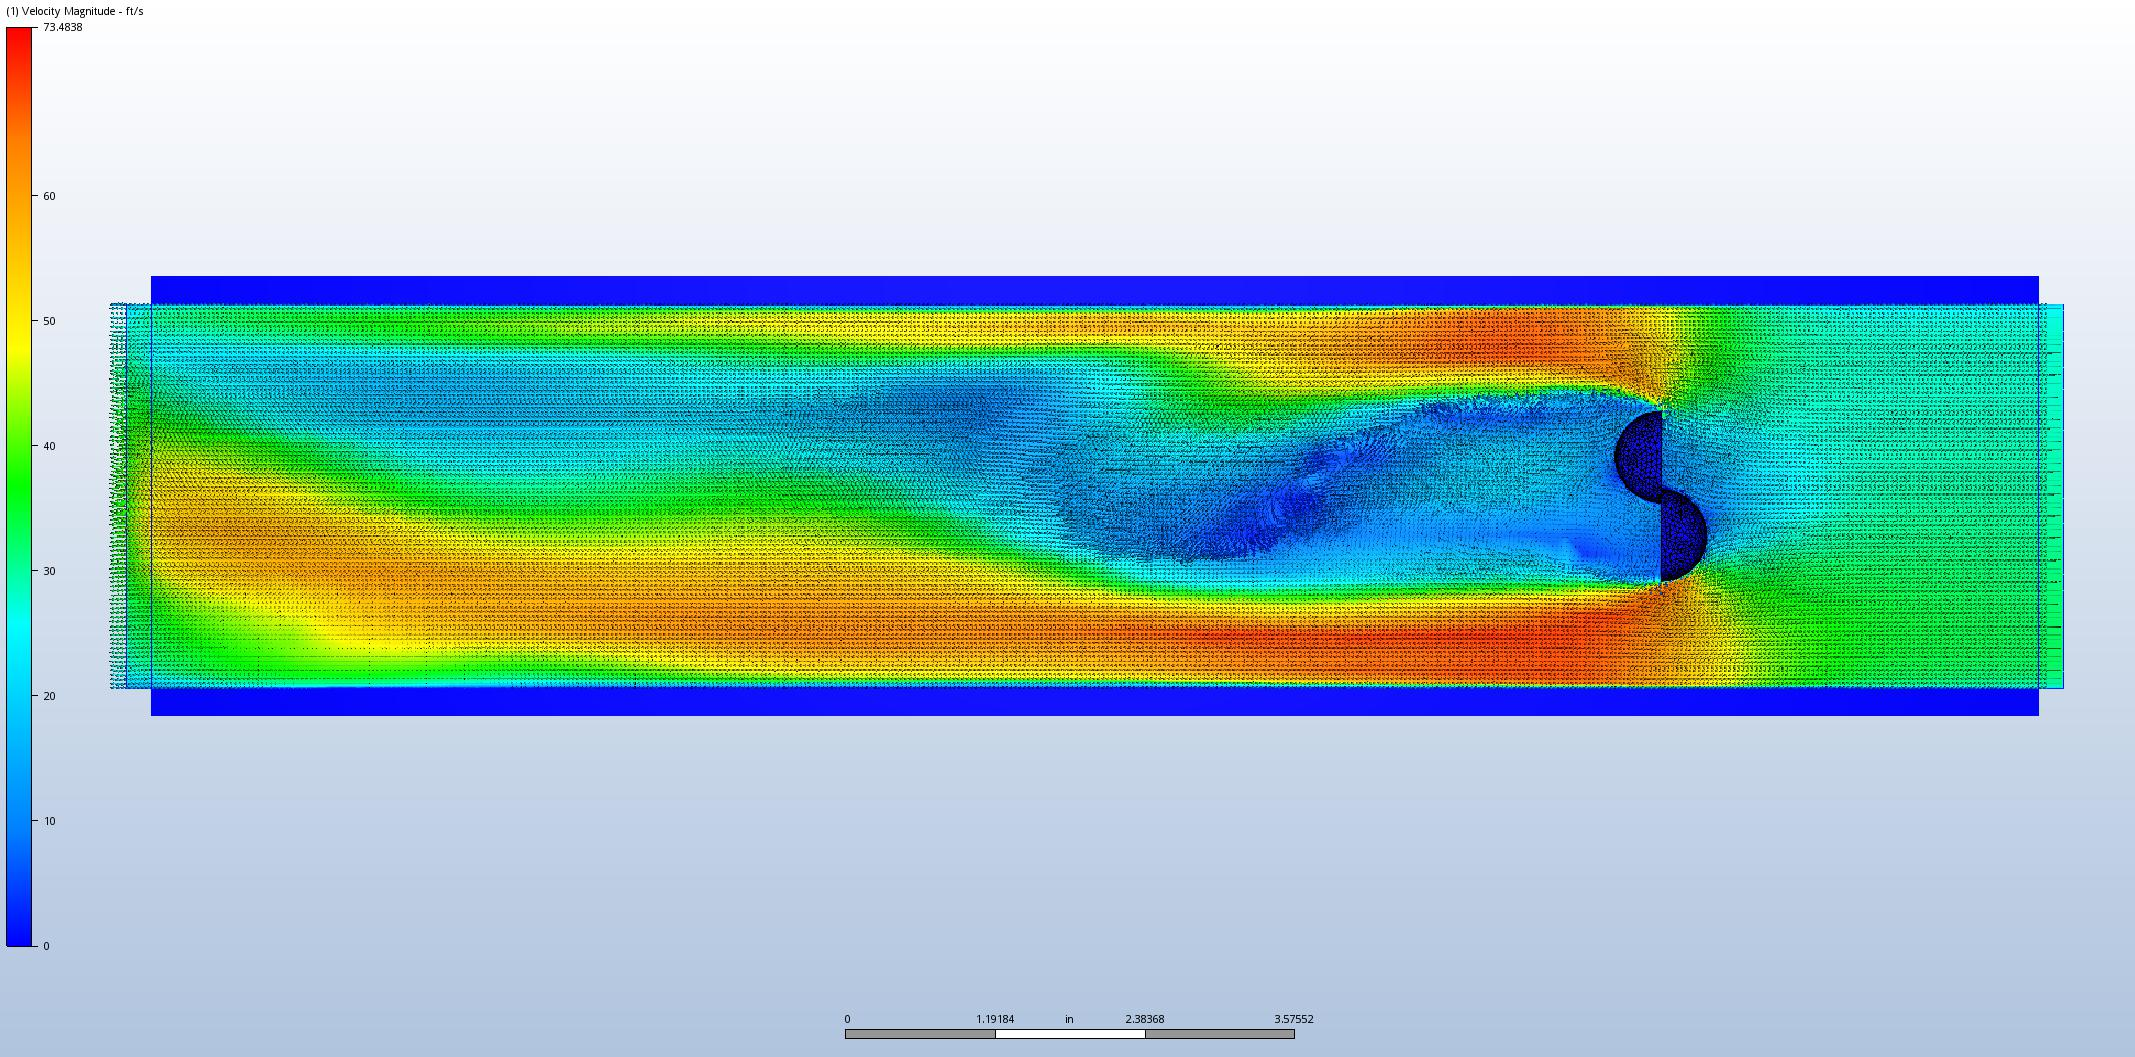
\includegraphics[width=0.6\textwidth]{CFD_Results/S_VM}
\caption[p1] {Simple Savonius - Velocity magnitude in x-y plane}
\label{ssv}
%\vspace{-0.4in}
\end{center}
\end{figure}
%%%%%%%%%%%%%%%%%%%%%
%%%%%%%%%%%%%%%%%%%%%
% % \vspace{25pt}
\begin{figure}[H]
\begin{center}
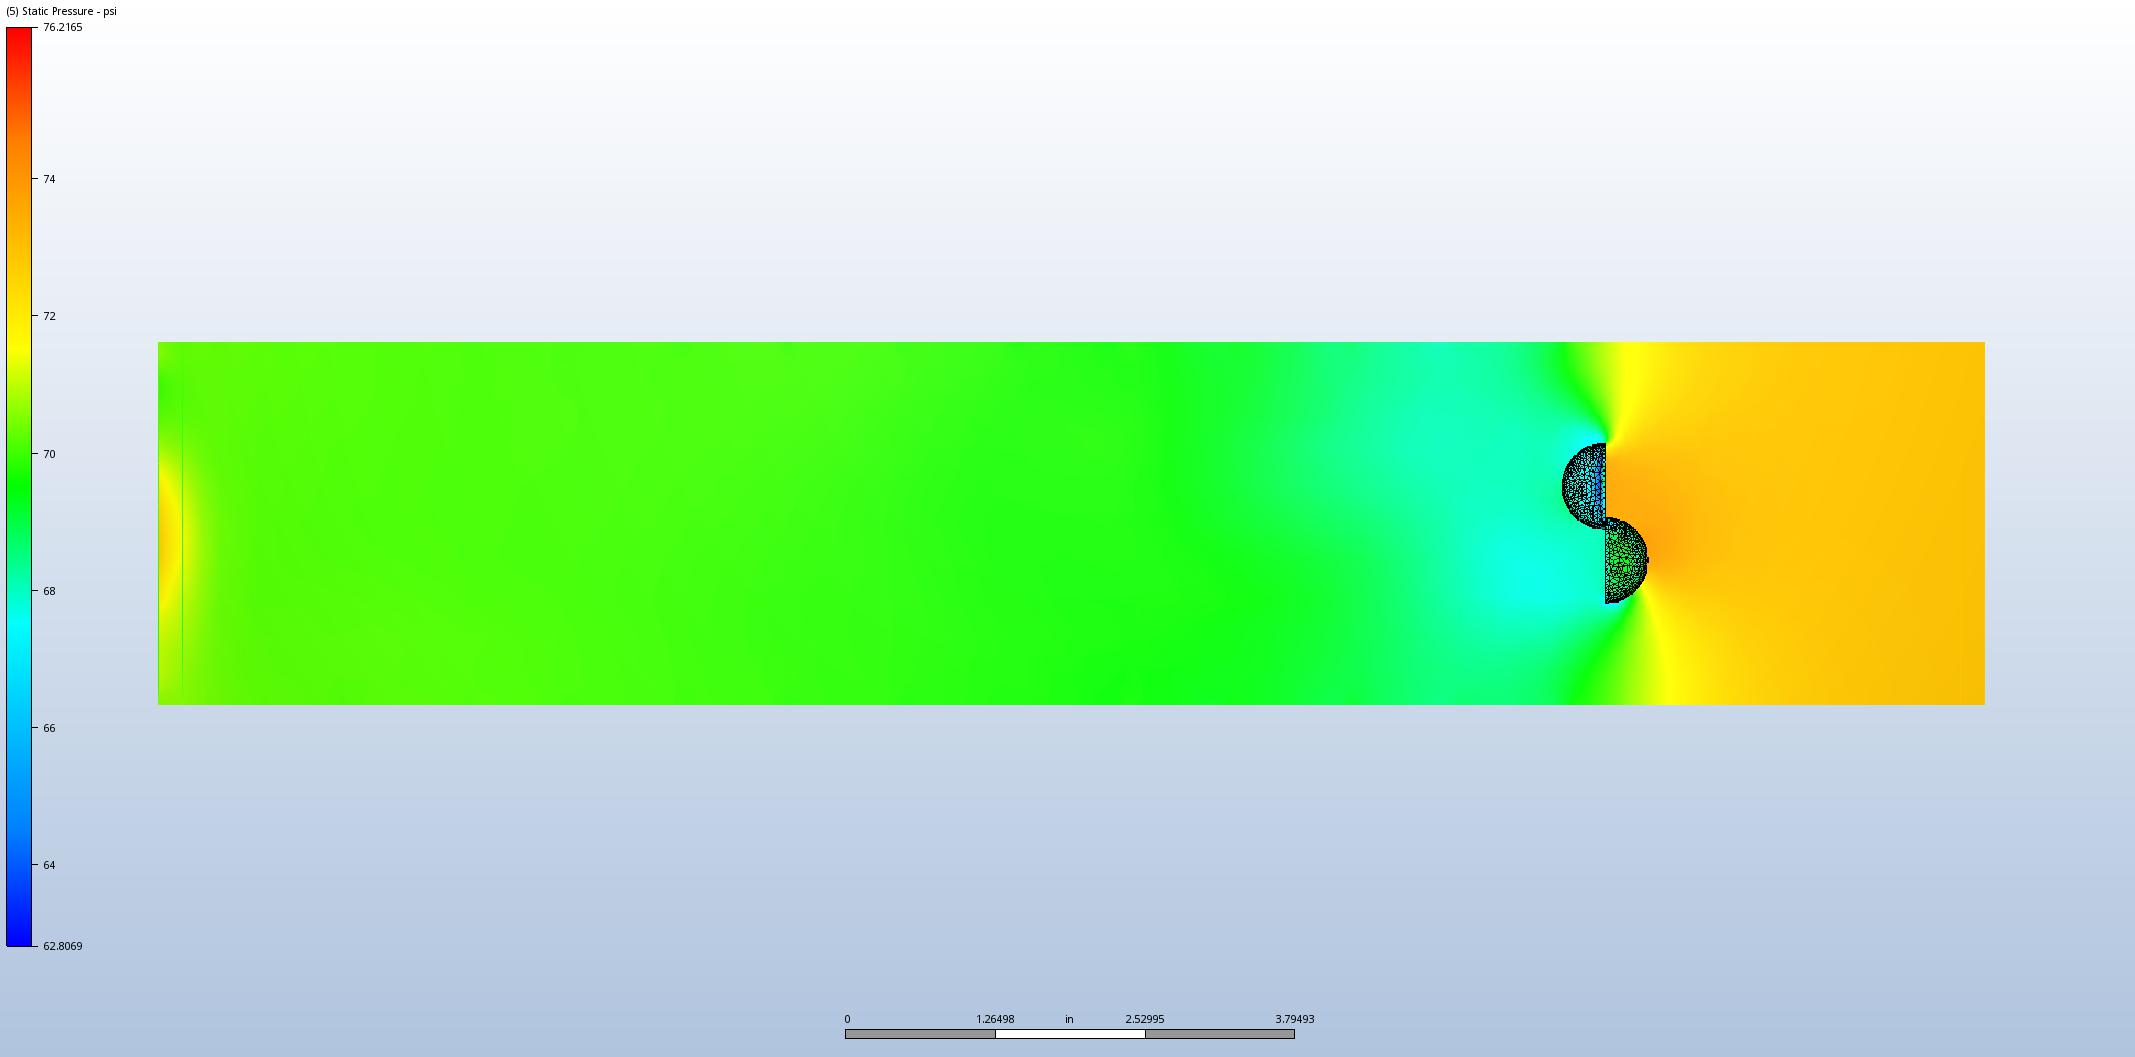
\includegraphics[width=0.6\textwidth]{CFD_Results/S_P}
\caption[p1] {Simple Savonius - Pressure differential in x-y plane}
\label{ssp}
%\vspace{-0.4in}
\end{center}
\end{figure}
%%%%%%%%%%%%%%%%%%%%%
%%%%%%%%%%%%%%%%%%%%%
% % \vspace{25pt}
\begin{figure}[H]
\begin{center}
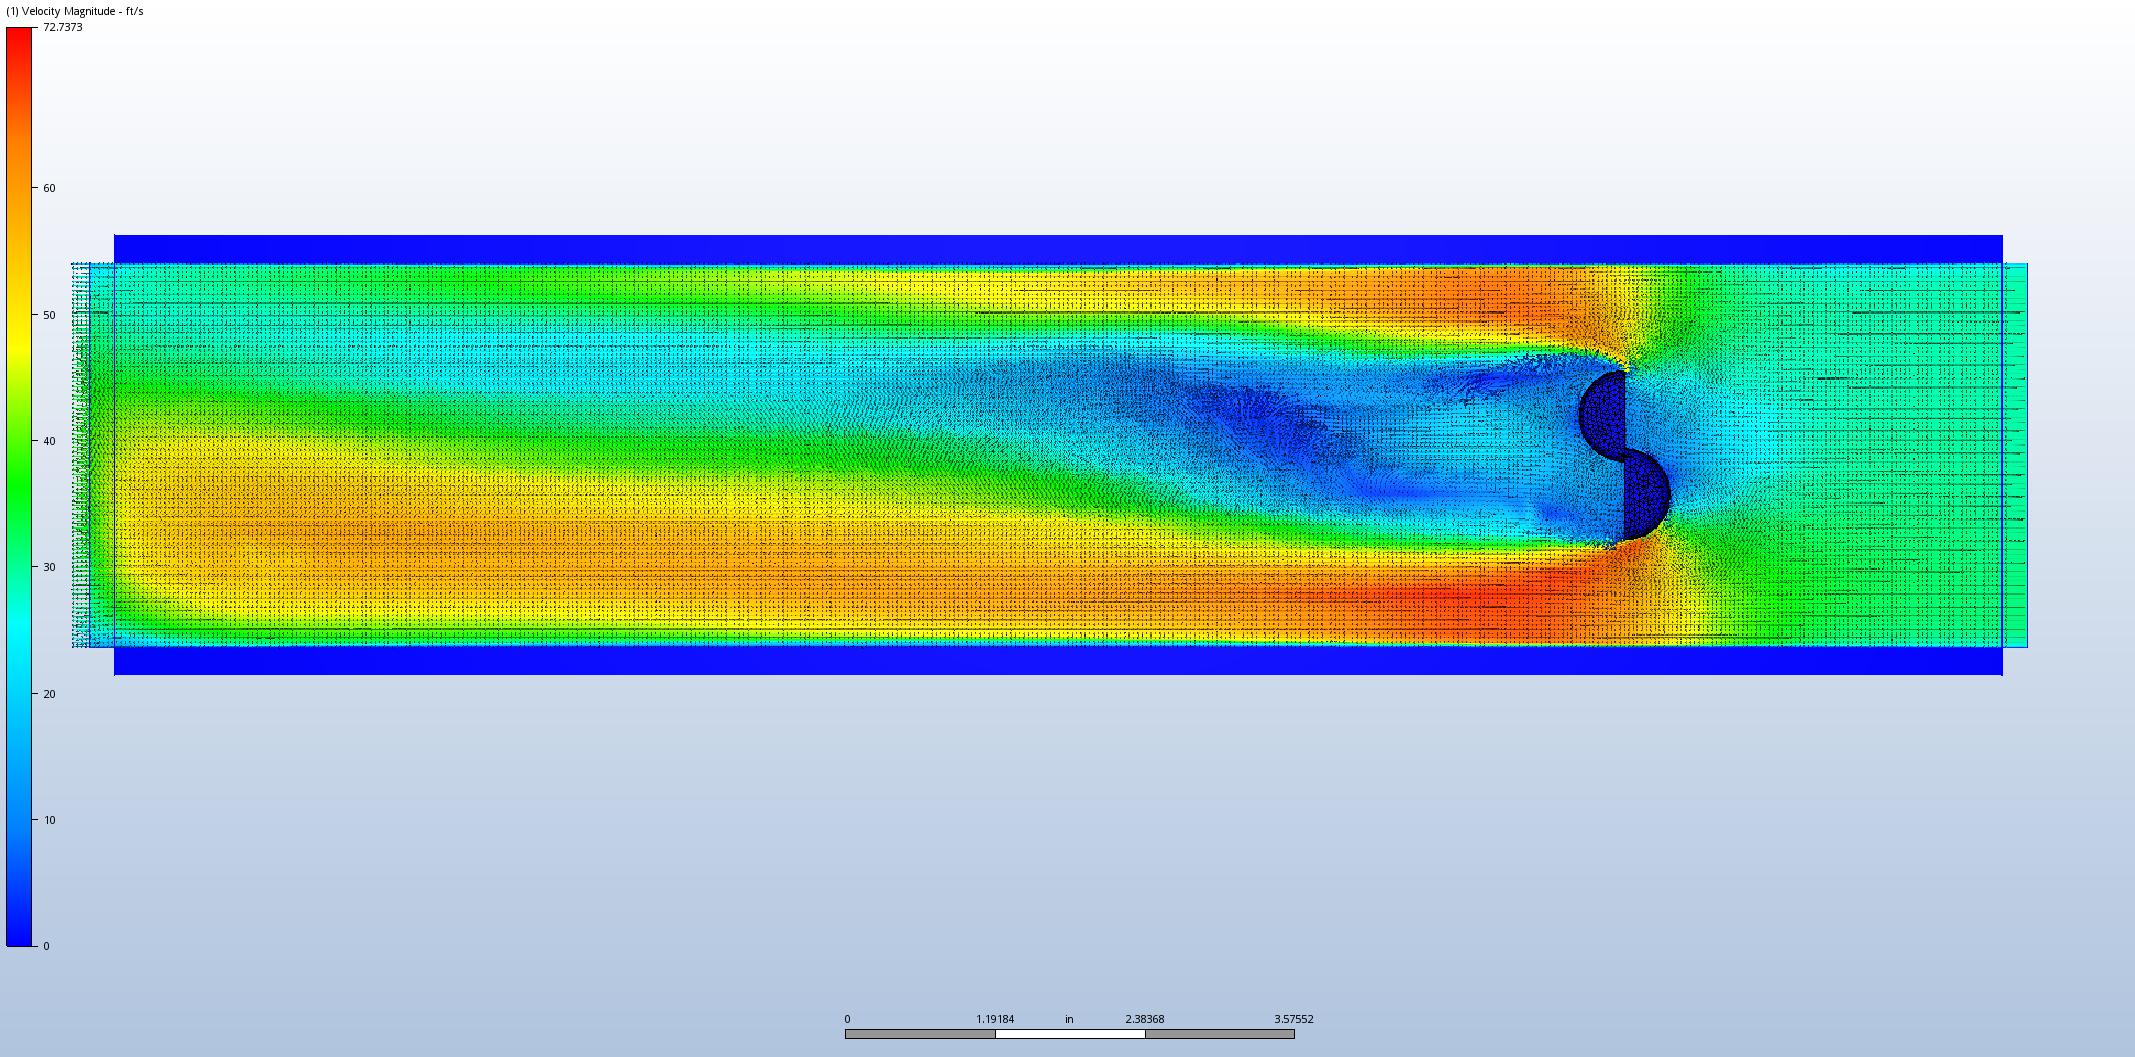
\includegraphics[width=0.6\textwidth]{CFD_Results/C_VM}
\caption[p1] {Crescent Savonius - Velocity magnitude in x-y plane}
\label{cvm}
%\vspace{-0.4in}
\end{center}
\end{figure}
%%%%%%%%%%%%%%%%%%%%%
%%%%%%%%%%%%%%%%%%%%%
% % \vspace{25pt}
\begin{figure}[H]
\begin{center}
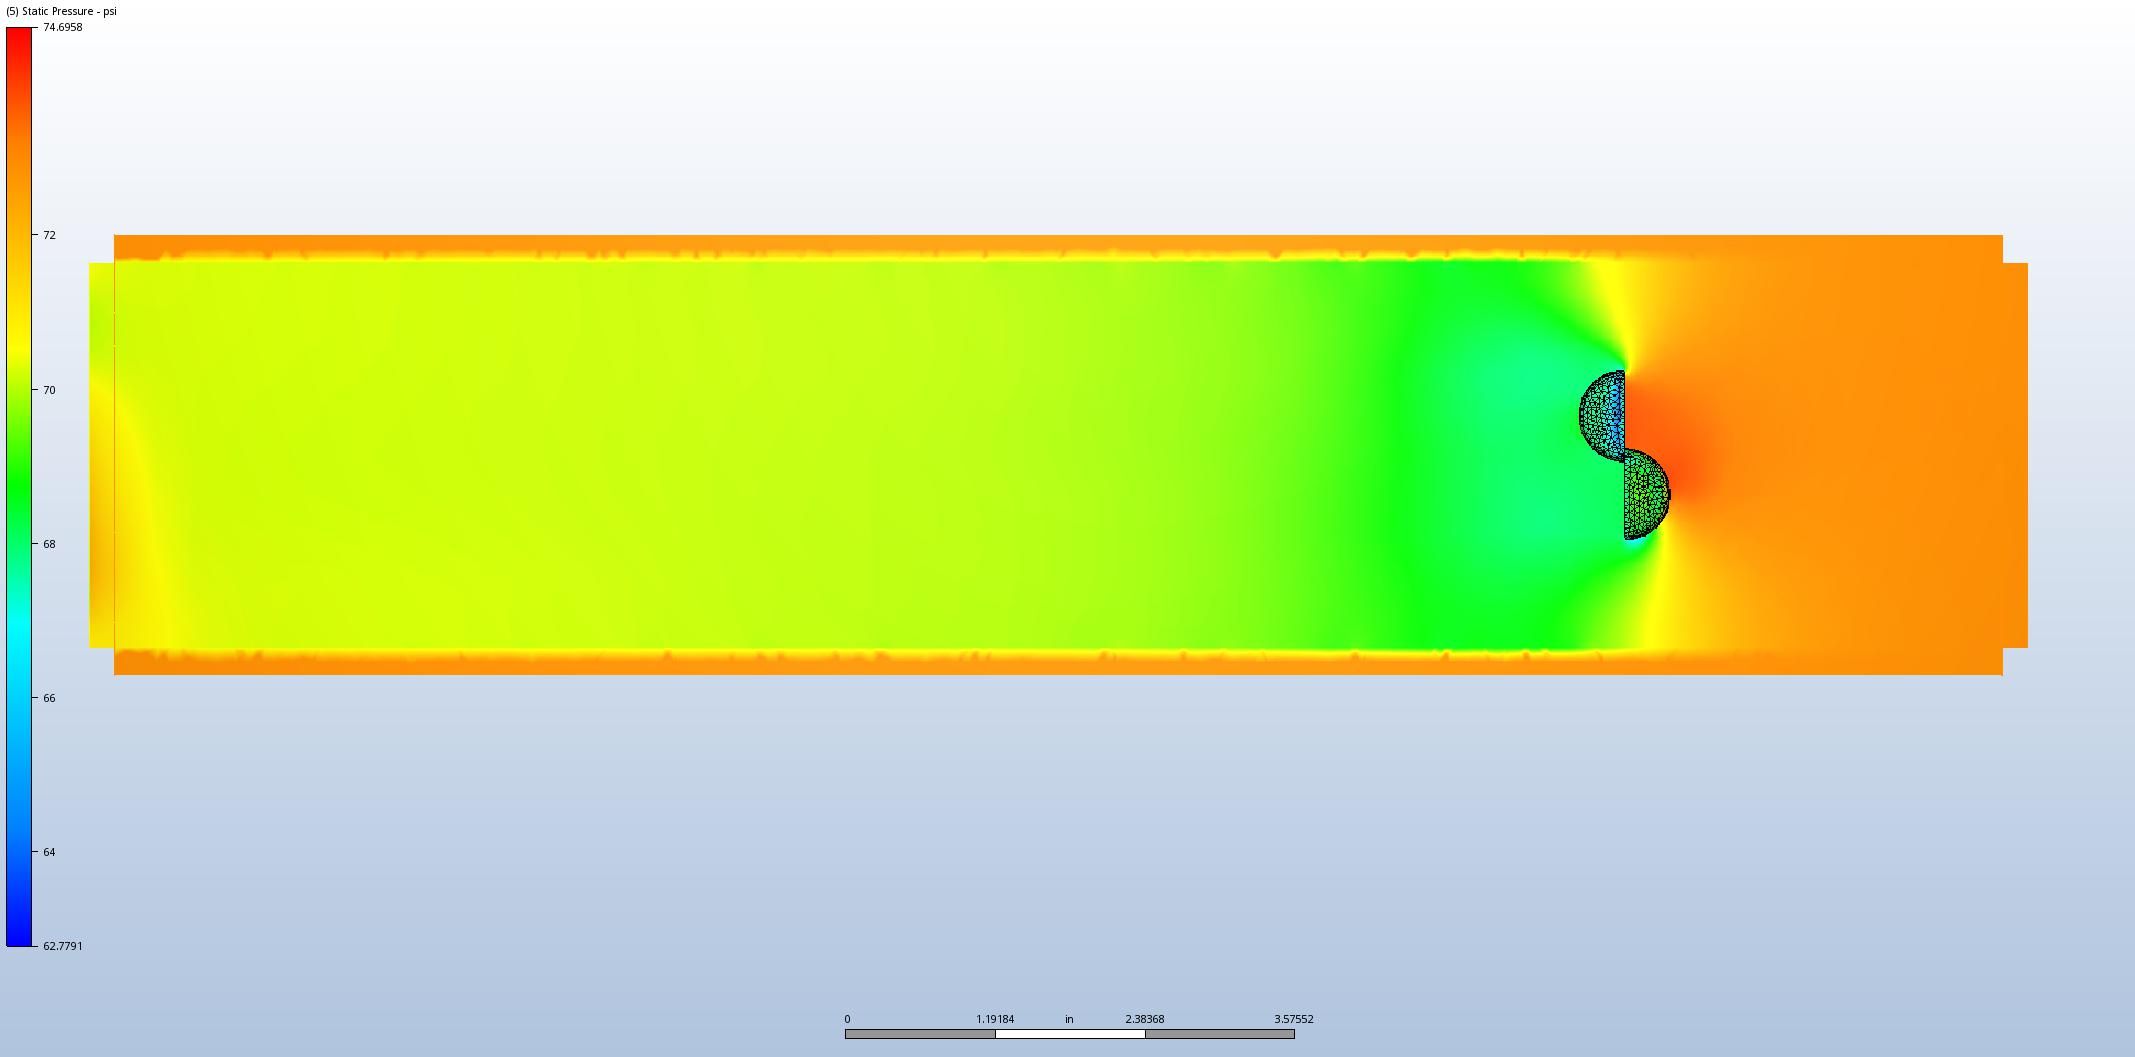
\includegraphics[width=0.6\textwidth]{CFD_Results/C_P}
\caption[p1] {Crescent Savonius - Pressure differential in x-y plane}
\label{cp}
% \vspace{-0.4in}
\end{center}
\end{figure}
%%%%%%%%%%%%%%%%%%%%%%%%%%%%%%%%%%%%%%%%%%%%%%%%%%%%%%%%%%%%%%%
%%%%%%%%%%%%%%%%%%%%%%%%%%%%%%%%%%%%%%%%%%%%%%%%%%%%%%%%%%%%%%%
%%%%%%%%%%%%%%%%%%%%%%%%%%%%%%%%%%%%%%%%%%%%%%%%%%%%%%%%%%%%%%%
\hspace{0.5 in}A comparison of the velocity magnitude and pressure differential results for both designs were plotted against one another and can be seen in Figures \ref{spvm} and \ref{sppd}. It can be observed that pressure differentials are nearly exact and the Crescent design's velocity magnitude is slightly higher than that of the Simple Savonius' by approximately 5 $\frac{ft}{s}$. Values extracted from the analysis were used to estimate potential power to be extracted using (\ref{eqn:mche_energy}).
%%%%%%%%%%%%%%%%%%%%%%%%%%%%%%%%%%%%%%%%%%%%%%%%%%%%%%%%%%%%%%%
%%%%%%%%%%%%%%%%%%%%%%%%%%%%%%%%%%%%%%%%%%%%%%%%%%%%%%%%%%%%%%%
%%%%%%%%%%%%%%%%%%%%%%%%%%%%%%%%%%%%%%%%%%%%%%%%%%%%%%%%%%%%%%%
\vspace{-0.1 in}
\begin{equation}
\dot{W} = \dot{V}[{\Delta P}+\frac{1}{2}\rho \Delta V^2]
\label{eqn:mche_energy}
\end{equation}
\vspace{-0.2 in}
%%%%%%%%%%%%%%%%%%%%%
\begin{figure}[H]
\begin{center}
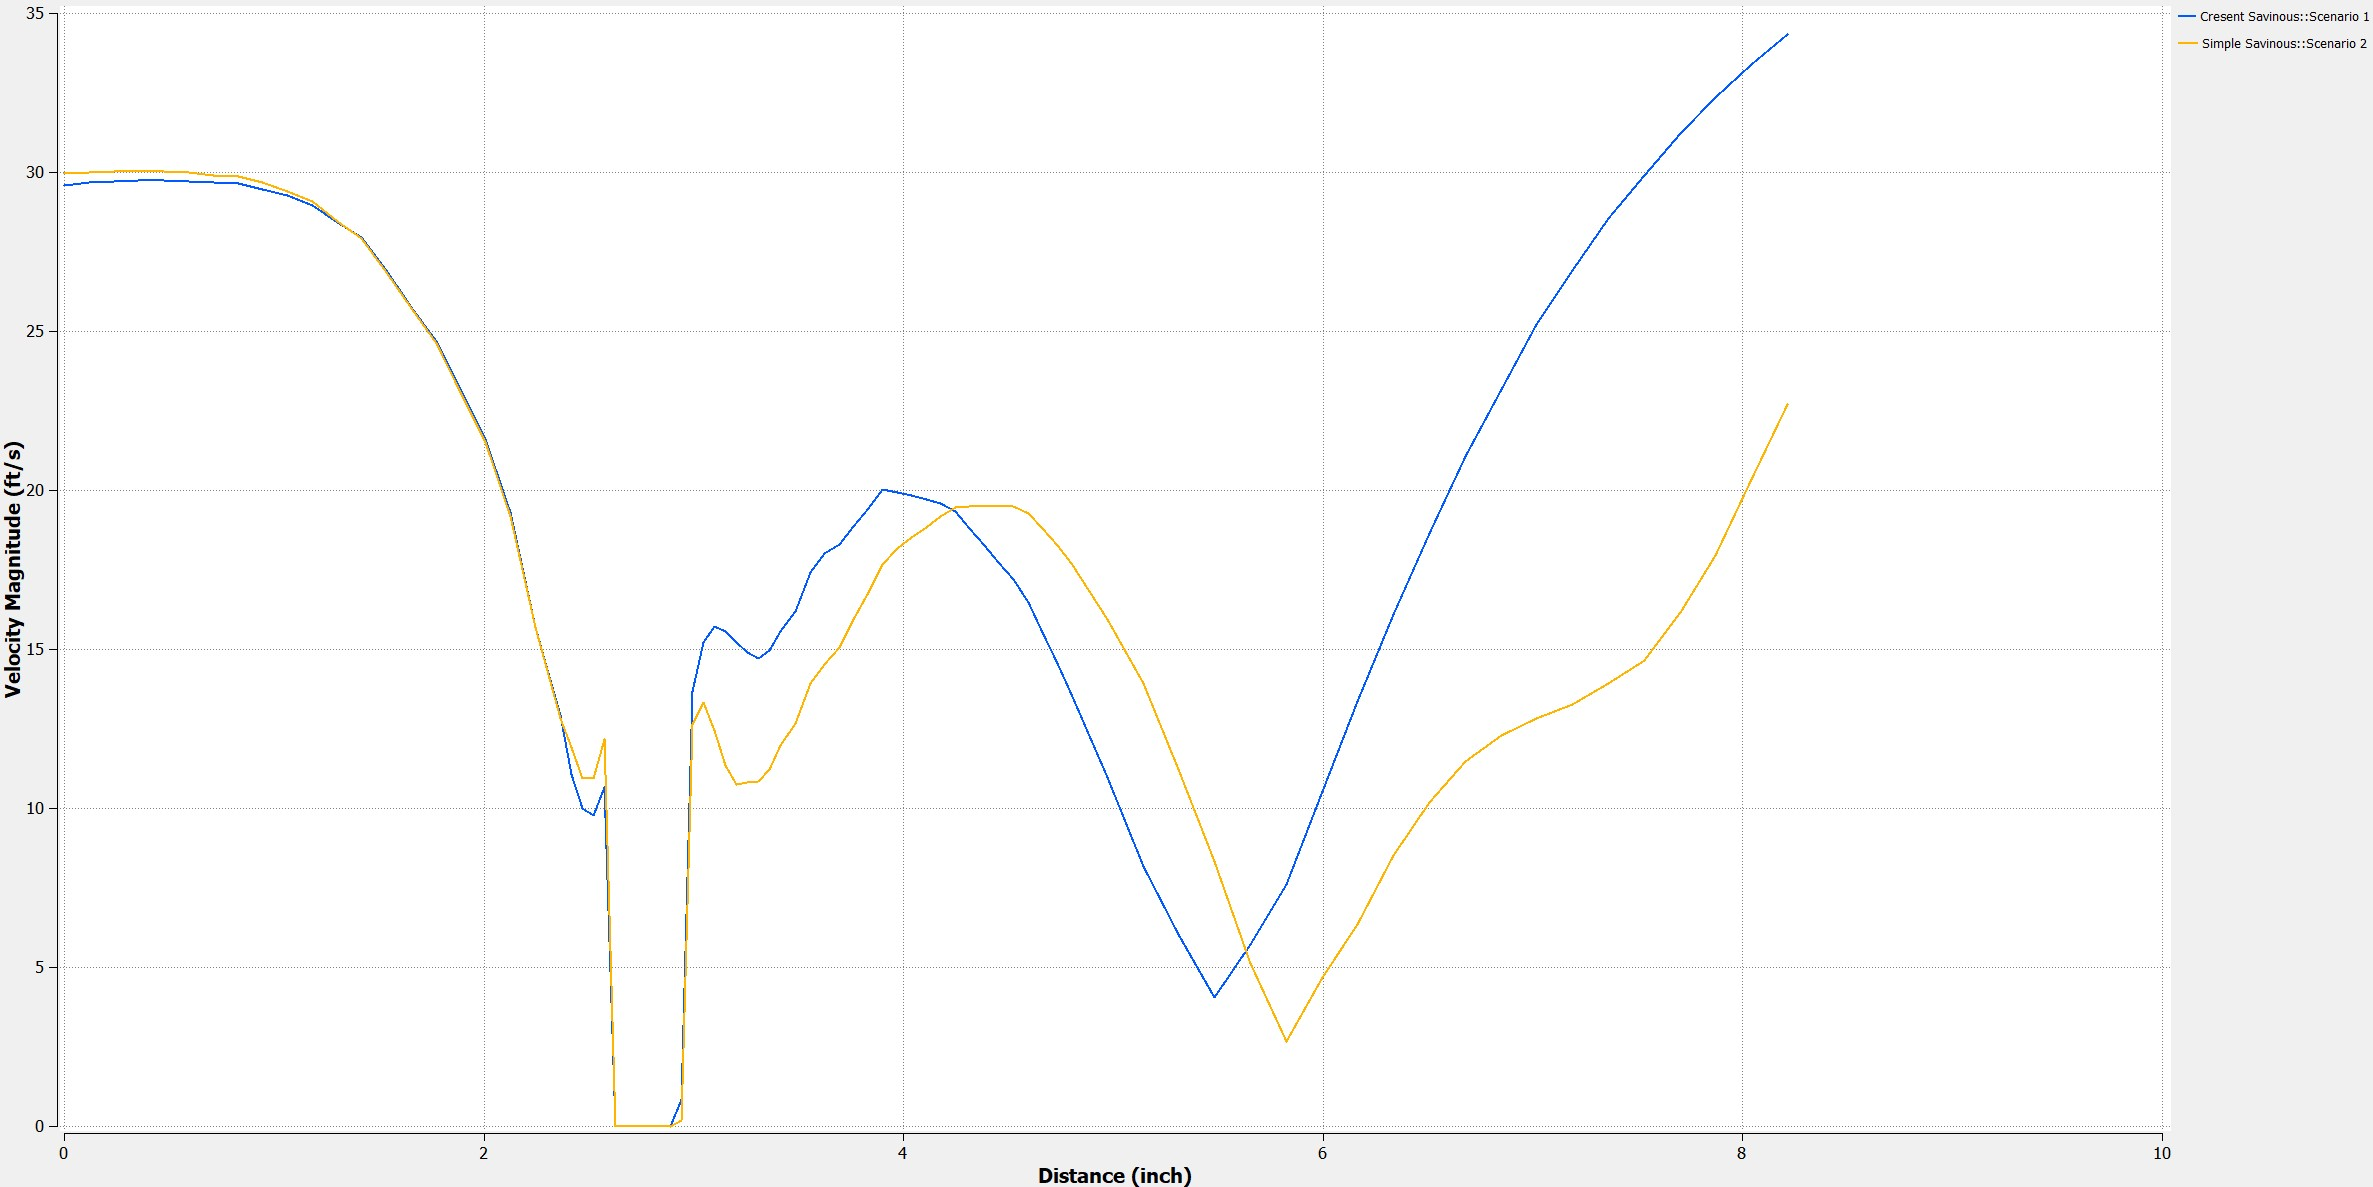
\includegraphics[width=0.6\textwidth]{spvm}
\caption[p1] {Summary comparison plot of velocity magnitude}
\label{spvm}
%\vspace{-0.4in}
\end{center}
\end{figure}
\begin{figure}[H]
\begin{center}
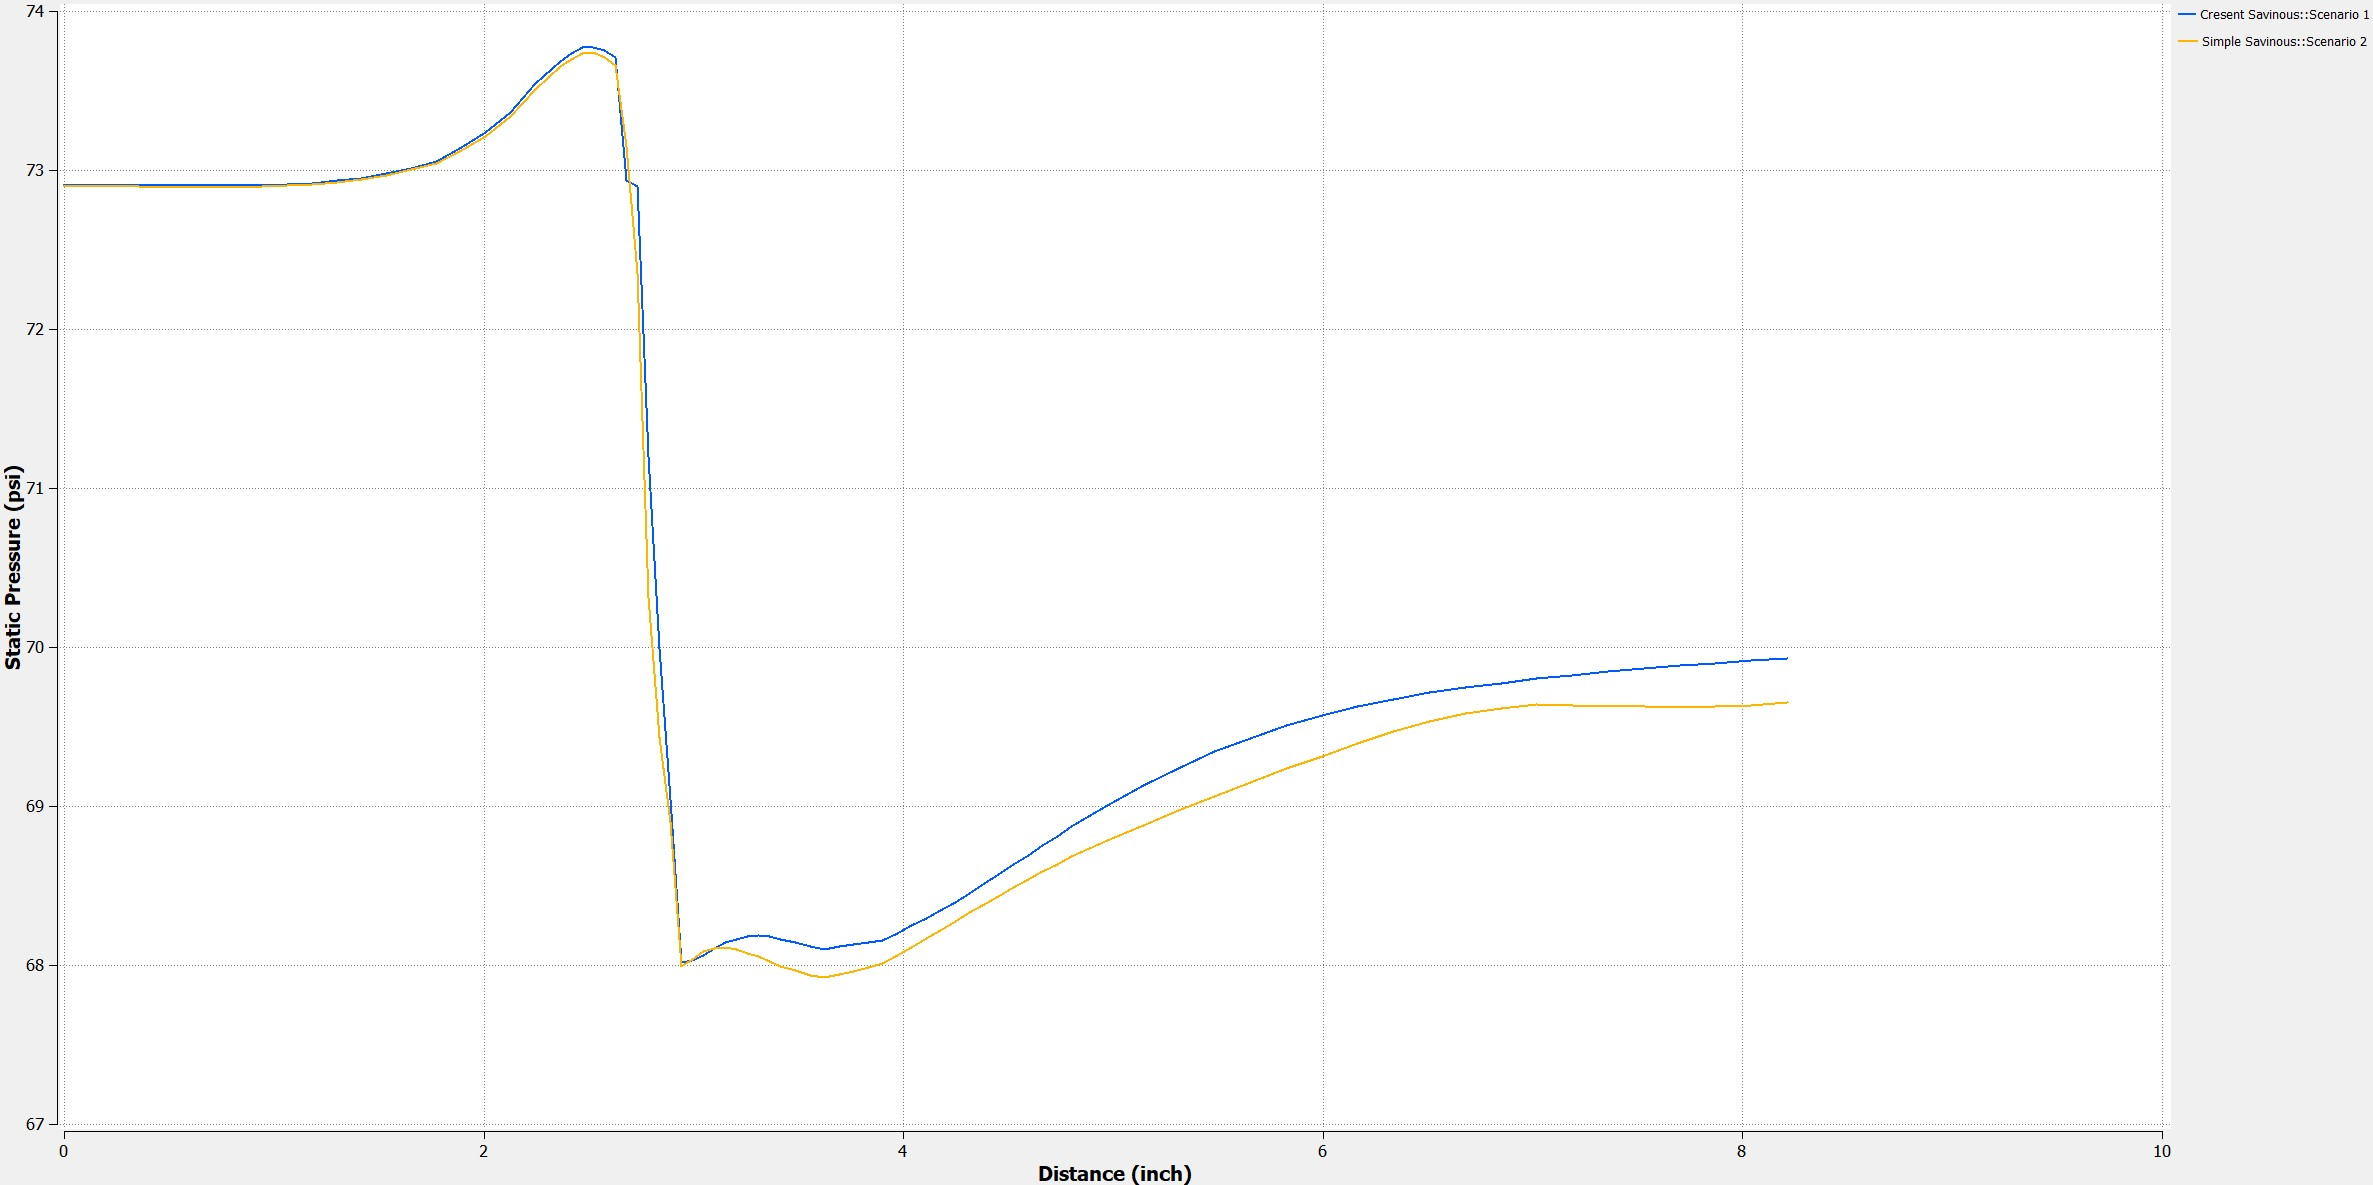
\includegraphics[width=0.6\textwidth]{sppd}
\caption[p1] {Summary comparison plot of pressure differential}
\label{sppd}
\end{center}
\end{figure}
%%%%%%%%%%%%%%%%%
\hspace{0.5 in}The resulted power potentially extracted was relatively the same, approximately 1,391 watts for the Simple Savonius and 1,397 watts for the Crescent Savonius design.

\hspace{0.5 in} The results discussed above provides reasonable data to conclude that the Crescent Savonius design is minimally more efficient than the Simple Savonius design. The data presented in this design report gives Stonewall the data needed to fully develop a profitable product.
%%%%%%%%%%%%%%%%%%%%%%%%%%%%%%%%%%%%%%%%%%%%%%%%%%%%%%%%%%%%%%%%%%%%%%%
%%%%%%%%%%%%%%%  PROJECT TIMETABLE   %%%%%%%%%%%%%%%%%%%%%%%%%%%%%%%%%%
%%%%%%%%%%%%%%%%%%%%%%%%%%%%%%%%%%%%%%%%%%%%%%%%%%%%%%%%%%%%%%%%%%%%%%%
%
% Identify duration of major tasks completed/remaining using the Gantt chart 
%
\vspace{-0.1in}
\section{Project Timetable}
\label{sec:Time}
\vspace{-0.2in}
\doublespacing

\hspace{0.5 in}Due to Stonewall changing the orientation of the insertion point, the diameter of the insertion point, and the pipe diameter the research and conceptual designs from the previous semester were no longer valid. Research and modeling of the new conceptual designs relating to the new customer requirements was completed in about three weeks. Initial CFD analyses were conducted on the multiple 3D blade designs and two designs showed promising results. Learning the functionality of the 3D program was time consuming, but became very beneficial for the overall success for this project. The duration of this task lasted for approximately three weeks. Simultaneously, preparation for the midterm report and presentation took place. After receiving valuable feedback from our midterm report and presentation, additional static CFD analyses were conducted on the turbine blade designs. This task took a considerable amount of time due to its complexity and lasted through the end of the April. The 3D printing of two prototypes was completed in a day using resources from the public library. Finally, the final report and presentation were completed in the final week. Following the Gantt chart was a valuable tool to ensure the group followed the projected timetable.
%%%%%%%%%%%%%%%%%%%%%%%%%%%%%%%%%%%%%%%%%%%%%%%%%%%%%%%%%%%%%%%%%%%%%%%
%%%%%%%%%%%%%%%  BUDGET   %%%%%%%%%%%%%%%%%%%%%%%%%%%%%%%%%%%%%%%%%%%%%
%%%%%%%%%%%%%%%%%%%%%%%%%%%%%%%%%%%%%%%%%%%%%%%%%%%%%%%%%%%%%%%%%%%%%%%
%
% List items purchased/to be purchased and approximate cost. 
%
\vspace{-0.2in}
\section{Budget}
\label{sec:Budget}
\vspace{-0.2in}
\doublespacing

\hspace{0.5 in}Stonewall did not set a strict budget for this project. However, due to no outside source of funding, decisions were made to minimize the total amount spent. With that being said an initial budget was estimated to be about 250 USD. This included the total sum of the cost for the 3D printer filaments, the testing equipment, and the hourly rate of 3D printing was given a plus or minus fifty percent contingency for unforeseen costs or expenses that may not be necessary.
    
Based on this preliminary budget and the plan of action going forward, a general idea of how much money was to be spent was understood. The final amount of money spent can be seen in Figure \ref{budget} below. This total includes the polylactic-acid 3D printer filament, the mini-generator and gearbox, the poster for the poster fair, and the cost of 3D printing. The cost of 3D printing ended up being free courtesy of the Lafayette Public Library provided that the filament was supplied. The total cost at the end of the project ended up being \$187.00, which is \$63.00 under the initial estimated budget.

\begin{figure}[ht]
\begin{center}
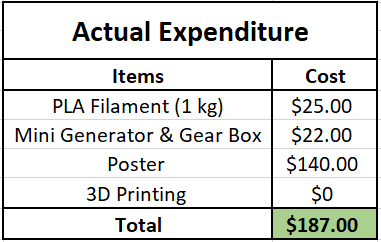
\includegraphics[width=0.5\textwidth]{SPEND.PNG}
\label{budget}
%\vspace{-0.4in}
\caption[p1] {Broken down expenditure}
\end{center}
\end{figure}
%%%%%%%%%%%%%%%%%%%%%%%%%%%%%%%%%%%%%%%%%%%%%%%%%%%%%%%%%%%%%%%%%%%%%%%
%%%%%%%%%%%%%%%  FACILITIES AND RESOURCES  %%%%%%%%%%%%%%%%%%%%%%%%%%%%
%%%%%%%%%%%%%%%%%%%%%%%%%%%%%%%%%%%%%%%%%%%%%%%%%%%%%%%%%%%%%%%%%%%%%%%
%
% Identify/list facilities and resources used or needed for project completion. 
%
\vspace{-0.2in}
\section{Facilities and Resources}
\label{sec:resources}
\vspace{-0.2in}
\doublespacing

\hspace{0.5 in}Stonewall allowed us to access their facilities on a 24/7 basis.  The facilities included conference rooms, computers and access to the servers and programs such as Autodesk Inventor, Autodesk CFD, and MathCad. Another facility and resource utilized was the Lafayette Public Library where free access to 3D print concepts was granted.

%%%%%%%%%%%%%%%%%%%%%%%%%%%%%%%%%%%%%%%%%%%%%%%%%%%%%%%%%%%%%%%%%%%%%%%
%%%%%%%%%%%%%%%  TEAM ORGANIZATION   %%%%%%%%%%%%%%%%%%%%%%%%%%%%%%%%%%
%%%%%%%%%%%%%%%%%%%%%%%%%%%%%%%%%%%%%%%%%%%%%%%%%%%%%%%%%%%%%%%%%%%%%%%
%
% List team structure and posts taken by each team member. Describe duties of each post taken by each team member. 
%
\vspace{-0.2in}
\section{Team Organization}
\label{sec:organization}
\vspace{-0.2in}
\doublespacing
%\hspace{0.5 in}
Alex Simpson, Team Captain- Fabricated weekly progress reports, scheduled team meetings, assisted in any areas that needed attention.

Blake Talbot, Computational Director- Responsible for hand calculations, 3-d modeling, and CFD analysis.

Andrew Boudreau, Financial Director- Responsible for recording budget for project, as well as researching cost for possible materials needed throughout the process

Nicholas Beall, Communications Director- Responsible for communicating with Stonewall, as well as other contacts that may have been necessary for this project.

Tyler LaCombe, Fabrication/Testing Director-Responsible for preparing physical testing of our prototype, since this phase is towards the very end of our project Tyler assisted in any department that needed attention.

\hspace{0.5in}Overall these titles were mostly arbitrary, many of the task completed for this project were done with every group member helping out in multiple areas.
%%%%%%%%%%%%%%%%%%%%%%%%%%%%%%%%%%%%%%%%%%%%%%%%%%%%%%%%%%%%%%%%%%%%%%%
%%%%%%%%%%%%%%%  REFERENCES  %%%%%%%%%%%%%%%%%%%%%%%%%%%%%%%%%%%%%%%%%%
%%%%%%%%%%%%%%%%%%%%%%%%%%%%%%%%%%%%%%%%%%%%%%%%%%%%%%%%%%%%%%%%%%%%%%%
\newpage
%
%
\begin{thebibliography}{9}
%
\bibitem{research} 
Bachant P, Wosnik M. Experimental Investigation of Helical Cross-Flow Axis Hydrokinetic Turbines, Including Effects of Waves and Turbulence. ASME. Fluids Engineering Division Summer Meeting\textit{, ASME-JSME-KSME 2011 Joint Fluids Engineering Conference: Volume 1, Symposia – Parts A, B, C, and D ():1895-1906. doi:10.1115/AJK2011-07020.} 

\bibitem{Fluids} 
Cengel, Y. A. and Cimbala, J. M., 2006.
\textit{Fluid Mechanics: Fundamentals and Applications, 3\textsuperscript{rd} Ed}. 
McGraw-Hill Higher Education, Boston, MA.


\end{thebibliography}

%%%%%%%%%%%%%%%%%%%%%%%%%%%%%%%%%%%%%%%%%%%%%%%%%%%%%%%%%%%%%%%%%%%%%%%
%%%%%%%%%%%%%%%  APPENDIX A  %%%%%%%%%%%%%%%%%%%%%%%%%%%%%%%%%%%%%%%%%%
%%%%%%%%%%%%%%%%%%%%%%%%%%%%%%%%%%%%%%%%%%%%%%%%%%%%%%%%%%%%%%%%%%%%%%%
\newpage

\section*{Appendix A}
\label{sec:a}
\vspace{0.2in}

% The code below is what creates the table.
\begin{table}[ht]
\label{table:parameters}
\begin{center}
\caption{Pipeline Conditions and Parameters}
\vspace{0.1in}
\begin{tabular}{ll}
\hline
\hline
Parameter & Value  \\
\hline
Standard Flow Rate, $Q$ & 525.451 $scfm$ \\
Actual Flow Rate, $Q_{act}$ & 90.255 $acfm$ \\
Gas Pressure, $P_{in}$ & 72.9 $psi$  \\
Gas Temperature, $T$ & 72.38 $^o F$ \\
Methane Gas Constant, $R_{g}$  & 3099 $\frac{ft-lb}{slug-R}$ \\
Pipe Inside Diameter, $ID$ & 3.06 $in.$ \\
Density of Gas, $\rho_{gas}$ & 0.136 $\frac{lb}{ft^3}$ \\[1ex]
\end{tabular}
\end{center}
\end{table}


\end{document}